
\chapter{Requirements Space}

\chapterintro*

The use of industrial wireless networks has been studied in many works in the literature and industry. However, no comprehensive survey of the whole problem space of industrial communications has been performed.   The following chapter provides some background into the evolving landscape of industrial wireless requirements.  It should be noted that the requirements perspective is often influenced by hype of the marketplace, and often the requirements that are stated are unrealistic or impossible to meet within reasonable price points.  First, and literature review is provided which was the result of the work presented by the thesis candidate in~\cite{CandellRW2017}.  This literature review will be followed by another distilled perspective provide in NIST 300-8~\cite{Montgomery2019} of which the candidate took a lead role in producing and leading.  Within that work, a picture of the wireless requirements landscape is provided based on inputs from the International Society of Automation (ISA) and the European Telecommunications Standards Institute (ETSI).  The work then provides a more distilled view of the requirements perspective with rationale.  This distilled perspective serves as both a state of the art of industrial user requirements viewed by ETSI and ISA, but it also serves as a major contribution by the candidate in that it provides validated requirements that are usable to build realistic and functional wireless systems.  This is ultimately the goal of performing a rigorous review of the requirements landscape and producing saner perspective.  A clearer concept of the requirements will not only allow for the development of realistic wireless systems, but it is also essential in the construction of more accurate models, the conduct of more effective testing, and better analysis the performance measurement data that results.

\section{Literature Review}\label{sec:litreview:academia}

In \cite{6248648}, the authors have introduced a comparison between the commercial and industrial communications networks where an industrial network has been divided to five different levels. These levels include field equipment, controller level, application, supervisory, and external networks. The differences in requirements between different levels are discussed. Moreover, three types of information are considered which are control, diagnostic, and safety information as described in \cite{4118467}. However all these levels of industrial networks are mentioned in \cite{6248648}, the article focuses only on the manufacturing and instrumentation communications and does not consider other types of communications networks that exist in industrial environments. Also, in \cite{What}, three levels of communications are considered which are device, control, and information levels. Moreover, the current wired industrial technologies for these levels are discussed briefly.

More works focused on the communications at the field devices level where sensing and control information is transfered. In \cite{7005074},  the communication between field devices has been studied where the requirements for a large number of nodes may not be achieved. The use of fieldbus solutions limit the scalability and resilience and hence industrial Ethernet capabilities are introduced in this article. Moreover, in \cite{Connectivity}, the communication for monitoring and control operations is discussed. A comparison between fieldbus technologies, industrial Ethernet, and wireless solutions is performed. The author has discussed the use of Wi-Fi, Bluetooth, ZigBee, and WirelessHART technologies in industrial applications. Similarly, the authors of \cite{6490786} considered the industrial communications networks requirements in process automation specifically at field devices level. Finally, in \cite{GE_Professional}, many case-studies are discussed for communication networks in industrial scenarios. Moreover, the design steps for these solutions are briefly discussed.

\section{Industry Requirements Perspectives}

In the following discussions, a presentation of different perspectives of various user requirements provided by industry is given based on industry reports from two noteworthy organizations.  This perspective differs from the perspectives provided by the academia in Section~\ref{sec:litreview:academia} in that contributors of these reports were individuals working directly within factory organizations or suppliers of products and services used by factory control engineers.  The first discussion in Section~\ref{sec:litreview:isa} focuses on the requirements work performed by the standards organization, the International Society of Automation.  The second discussion given in Section~\ref{sec:litreview:etsi} focuses on work performed by the European Telecommunications Standards Institute regarding high-reliabilty, low-latency communications requirements for industrial applications, and in particular for the 5th generation wireless evolution known as 5G.  The third discussion provided in Section~\ref{sec:litreview:industry} while an academic article was the result of research performed by engineers developing wireless products for high-performance wireless networks used to control industrial operations by latency constraints within the microsecond range.  Finally, a consolidated and actionable perspective is provided in Section~\ref{sec:litreview:nist} which serves as both background material and contribution by the thesis candidate.  The consolidated perspective of the requirements were useful in the development of the SysML model presented in Chapter~\ref{chapter:sysml}.

\subsection{ISA Requirements Perspective}\label{sec:litreview:isa}

The International Society of Automation (ISA) is a non-profit standardization body that produced Wireless User Requirements for Factory Automation [10]. ISA provided classes that categorized industrial applications and use cases, and assigned wireless user requirements for latency, jitter, and block error rate (BLER). Table~\ref{soa:isa-classes}, adapted from~\cite{ISATR100-2011}, provides usage classes with their respective descriptions; these classes are grouped by domain, in factory automation use cases. It is important to note that the “Factory Automation Use Cases” column references “Clauses” which describe applications in the usage classes in detail and are not discussed in this report. The Clauses discuss various industrial applications and such applications apply to different classes. For example, robot end-effectors for Class 1, track-mounted equipment and rotary equipment for Class 2, track-mounted equipment and rotary equipment, but with a human in the loop for Class 3; torque and gauge tools, mobile material containers, mobile high value assets (molds, dies, etc.), and mobile test and calibration fixtures for Class 4. Note that the report references similar applications for Class 4 as for Class 5, except with the purpose of logging, downloading, and uploading; also note that Class 0, was not discussed. The ISA requirements, adapted in Table~\ref{soa:isa-reqts-persp}, define BLER as the probability of an erroneous block received at the application layer. It should be noted that all usage classes have a requirement of $10^{-9}$ BLER, an assumed requirement, without justification, in the ISA’s report. 

% Table generated by Excel2LaTeX from sheet 'ETSI and ISA'
\begin{table}[!tb]
	\centering
	\caption{ISA Descriptions of Wireless Requirements Classes}
	% Table generated by Excel2LaTeX from sheet 'ETSI and ISA'

	\begin{adjustbox}{width=\columnwidth,center}
		
	% Table generated by Excel2LaTeX from sheet 'ETSI and ISA'
	\begin{tabular}{|l|l|p{10.645em}|p{10em}|}
		\toprule
		\multicolumn{1}{|p{6.355em}|}{\textbf{Domain}} & \multicolumn{1}{p{13.07em}|}{\textbf{Usage Class}} & \textbf{Description} & \textbf{Factory Automation Use Cases} \\
		\midrule
		\multicolumn{1}{|l|}{\multirow{2}[2]{*}{Safety}} & \multicolumn{1}{l|}{\multirow{2}[2]{*}{Class 0:  Emergency action}} & \multirow{2}[2]{*}{Always critical } & \multicolumn{1}{l|}{\multirow{2}[2]{*}{}} \\
		&       & \multicolumn{1}{l|}{} & \multicolumn{1}{l|}{} \\
		\midrule
		\multicolumn{1}{|l|}{\multirow{8}[6]{*}{Control}} & \multicolumn{1}{l|}{\multirow{2}[2]{*}{Class 1:  Closed loop regulatory control}} & \multirow{2}[2]{*}{Often critical } & \multirow{2}[2]{*}{Clause 5.3 } \\
		&       & \multicolumn{1}{l|}{} & \multicolumn{1}{l|}{} \\
		\cmidrule{2-4}      & \multicolumn{1}{l|}{\multirow{3}[2]{*}{Class 2:  Closed loop supervisory control}} & \multirow{3}[2]{*}{Usually non-critical } & Clause 5.4  \\
		&       & \multicolumn{1}{l|}{} & Clause 5.5  \\
		&       & \multicolumn{1}{l|}{} & \multicolumn{1}{l|}{} \\
		\cmidrule{2-4}      & \multicolumn{1}{l|}{\multirow{3}[2]{*}{Class 3:  Open loop control}} & \multirow{3}[2]{*}{Human in the loop } & Clause 5.4  \\
		&       & \multicolumn{1}{l|}{} & Clause 5.5  \\
		&       & \multicolumn{1}{l|}{} & \multicolumn{1}{l|}{} \\
		\midrule
		\multicolumn{1}{|l|}{\multirow{9}[4]{*}{Monitoring }} & \multicolumn{1}{l|}{\multirow{5}[2]{*}{Class 4:  Alerting}} & Short-term operational  & Clause 5.6  \\
		&       & consequence (e.g., event-based  & Clause 5.7  \\
		&       & maintenance)  & Clause 5.8  \\
		&       & \multicolumn{1}{l|}{} & Clause 5.9  \\
		&       & \multicolumn{1}{l|}{} & \multicolumn{1}{l|}{} \\
		\cmidrule{2-4}      & \multicolumn{1}{l|}{\multirow{4}[2]{*}{Class 5:  Logging, Downloading, and Uploading}} & No immediate operational  & Clause 5.6  \\
		&       & consequence (e.g., history  & Clause 5.7  \\
		&       & collection, sequence of events,  & Clause 5.8  \\
		&       & preventive maintenance)  & Clause 5.9  \\
		\bottomrule
	\end{tabular}%

	\end{adjustbox}

	\label{soa:isa-classes}%
\end{table}%


% Table generated by Excel2LaTeX from sheet 'ETSI and ISA'
\begin{table}[!tb]
	\centering
	\caption{ISA Wireless Requirements Perspective}
	\label{soa:isa-reqts-persp}%

	% Table generated by Excel2LaTeX from sheet 'ETSI and ISA'
	\begin{tabular}{|p{10.57em}|p{5.855em}|p{5.855em}|p{5.855em}|}
		\toprule
		\textbf{Use Case Class} & \textbf{Latency (ms)} & \textbf{Jitter (\%)} & \textbf{BLER} \\
		Class 0 & ND    & ND    & ND \\
		\midrule
		Class 1 & \multicolumn{1}{l|}{10} & $\pm10$ & $10^{-9}$ \\
		\midrule
		Class 2 and 3 & 10 to 100 & $<10$ & $10^{-9}$ \\
		\midrule
		Class 4 and 5 & 100 avg. & $\pm10$ & $10^{-9}$ \\
		\bottomrule
	\end{tabular}%
\end{table}%


\subsection{ETSI Requirements Perspective}\label{sec:litreview:etsi}

The European Telecommunications Standards Institute (ETSI) produced a requirements report titled Reconfigurable Radio Systems (RRS); Feasibility study on temporary spectrum access for local high-quality wireless networks [11]. The ETSI report included a detailed table, reproduced here in Table 3, which categorized specific industrial scenarios and listed certain requirement metrics such as latency, reliability, data rate, packet size, communication range, device mobility, device density, and energy efficiency. We find the ETSI report to be very detailed; however, justification of specific values and their derivations are not disclosed.

ETSI’s industrial wireless communications requirements are separated into different sections, depending on the application. Under Monitoring and Diagnostics, the application is focused on remote sensors that do not have strict latency or reliability requirements, compared to other applications. The column, Condition Monitoring, includes applications that report physical parameters, such as temperature, humidity, vibration, acceleration, etc., and the column has similar wireless network requirements to Process Automation. In discrete manufacturing, a countable number of items are produced which may take many steps to complete. In discrete manufacturing, machine tools, robots, sensors, and programmable logic controllers (PLCs) exchange small packets with short intervals, which requires low-latency communications. Motion Control has more strict latency requirements than general discrete manufacturing. Examples for Motion Control include a controller for an electric motor in an assembly line or a hydraulic cylinder controller for a press~\cite{etsi103588}.

The Logistics and Warehouse category is separated into mobile vehicles, automated guided vehicles (AGV) and static systems such as cranes. AGVs can be mobile robots, transport vehicles, and mobile working platforms. It is stated that a latency of 15 ms – 20 ms and a reliability requirement of $10^{-6}$ should be ensured. The General subcategory for “Logistics and Warehouse” is not discussed or justified within the ETSI report. Process Automation typically involves chemical processes engineering, for example, oil and gas production or the generation of electricity. In the Process Automation category, steps are sequential, continuous, and irreversible. Process Automation applications need deterministic delivery of transmissions, thus, the relaxed latency requirements and reliability of $10^{-5}$. The Augmented Reality category includes computer-assisted extension of reality. The Functional Safety category requires high reliability ($10^{-9}$) and low latency of 10 ms. Safety is critical to protect people, machines, and production environments, hence the stricter performance requirements. 

\begin{table}[!tb]
	\centering
	\caption{ETSI Industrial Wireless Requirements Perspective}
	\label{soa:ets-reqts-persp}	
	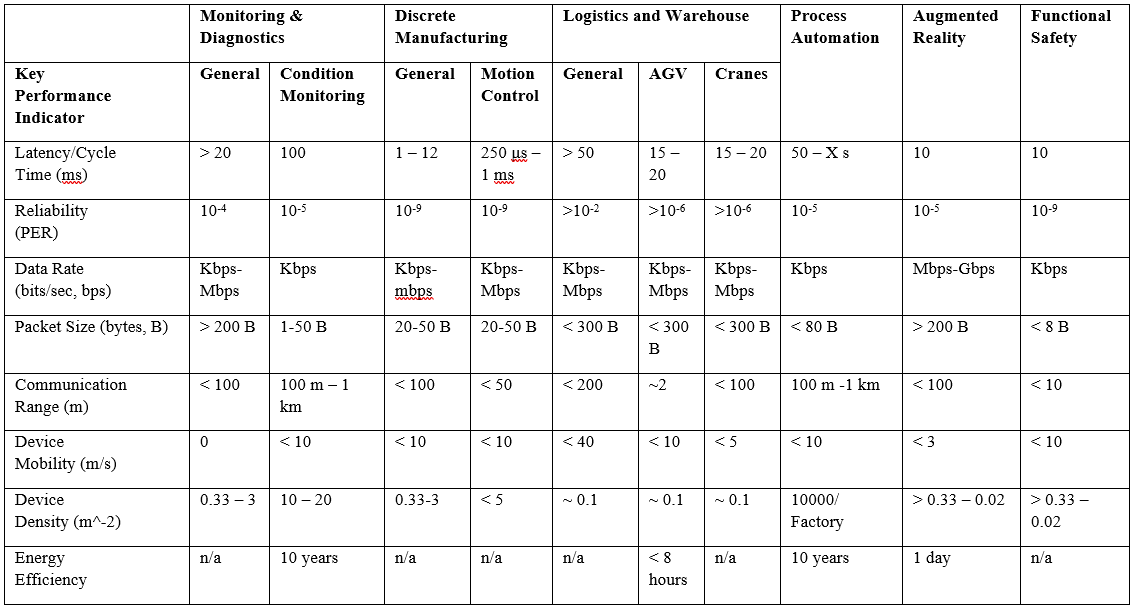
\includegraphics[width=\textwidth]{chapter-soa/etsi-reqts}
\end{table}

\section{An Industry Requirements Perspective}\label{sec:litreview:industry}

% Table generated by Excel2LaTeX from sheet 'FromKarl2019'
\begin{table}[!tb]
	\centering
	\caption{An Industry Requirements Perspective of Different Industrial Communication Scenarios}
	\label{soa:industry-reqts-persp}%
	
% Table generated by Excel2LaTeX from sheet 'Industry'
\begin{tabular}{|p{7.5em}|p{4.215em}|p{4.215em}|p{4.215em}|p{4.215em}|}
	\toprule
	\textbf{Scenario} & \textbf{\# of nodes} & \textbf{Update rate, Hz} & \textbf{Goodput, bps} & \textbf{System range, m} \\
	\midrule
	Building Automation & $10^{2}-10^{3}$ & $10^{-1}$ & $10^{3}-10^{4}$ & 10-100 \\
	\midrule
	Process Automation & $10^{2}-10^{3}$ & \multicolumn{1}{l|}{10} & $10^{5}-10^{6}$ & 10-100 \\
	\midrule
	Factory Automation & $10^{2}-10^{3}$ & $10^{3}$ & $10^{7}-10^{8}$ & 10-100 \\
	\midrule
	Power Systems Automation & $10^{1}-10^{2}$ & $10^{4}$ & $10^{7}-10^{8}$ & $10^{2}-10^{3}$ \\
	\midrule
	Power Electronics Control & $10^{2}-10^{3}$ & $10^{5}$ & $10^{9}-10^{10}$ & 10-100 \\
	\bottomrule
\end{tabular}%

	
\end{table}%

Another industry perspective presented in~\cite{Luvisotto2017}, targeted ultra-high-performance wireless for various scenarios ranging from building automation to the switching of power electronics equipment. An example of system-level requirements for different industrial communication scenarios is captured in Table~\ref{soa:industry-reqts-persp}. The scenario Building Automation consists of all control operations performed within buildings, such as lighting, heating, surveillance, energy management, etc. Process Automation is involved in chemical, mining, oil, and metallurgic processes. \textit{Factory Automation} is a general term referring to the factory production line, such as assembly and packaging. More demanding scenarios include \textit{Power Systems Automation} in which control for power distribution is performed. \textit{Power Electronics Control} focuses on the synchronized control of power electronic devices. All these scenarios have distinct requirements. Luvisotto states that for a wireless high performance (HP) system, a packet error rate (PER) of $10^{-9}$ is perceived as tolerable~\cite{Luvisotto2017}. It is important to clarify this PER is at the application layer and it is possible to have a PER of $10^{-1}$ at the physical layer and still achieve $10^{-8}$ at the application layer with transmission and information redundancy. It was proposed in the paper that a latency requirement of $10{\mu}s$ is targeted for Wireless-HP. It is stated that \textit{Factory Automation}, \textit{Power Systems Automation}, and \textit{Power Electronics Control} are the scenarios where their particular technology is applicable. The power electronics industry is very distinctive in the difficulty in meeting their challenges requirements; however, these requirements are not typical of all industry scenarios.

\subsection{NIST Validated Requirements Perspective}\label{sec:litreview:nist}

% Table generated by Excel2LaTeX from sheet 'FromKarl2019'
\begin{table}[!tb]
	\centering
	\caption{NIST Validated Wireless Requirements Perspective}
	\label{soa:nist-reqts-persp}%
	
	% Table genera% Table generated by Excel2LaTeX from sheet 'FromKarl2019'
	\begin{tabular}{|p{5.715em}|p{4.855em}|l|l|l|l|l|}
		\toprule
		\multicolumn{2}{|p{10.57em}|}{\textbf{User Requirement}} & \multicolumn{1}{p{4.355em}|}{\textbf{Class 0:}} & \multicolumn{1}{p{4.355em}|}{\textbf{Class 1:}} & \multicolumn{1}{p{4.355em}|}{\textbf{Class 2:}} & \multicolumn{1}{p{4.355em}|}{\textbf{Class 3:}} & \multicolumn{1}{p{4.355em}|}{\textbf{Class 4:}} \\
		\midrule
		\multirow{2}[4]{*}{Latency (ms)} & Typical & 4     & 4     & 20    & 4     & 50 \\
		\cmidrule{2-7}\multicolumn{1}{|l|}{} & Minimum & 0.5   & 0.25  & 4     & 0.5   & 4 \\
		\midrule
		Reliability & Typical & \multicolumn{1}{p{4.355em}|}{$10^{-7}$} & \multicolumn{1}{p{4.355em}|}{$10^{-7}$} & \multicolumn{1}{p{4.355em}|}{$10^{-7}$} & \multicolumn{1}{p{4.355em}|}{$10^{-7}$} & \multicolumn{1}{p{4.355em}|}{$10^{-6}$} \\
		\cmidrule{2-7}(Pr. Loss) & Minimum & \multicolumn{1}{p{4.355em}|}{$10^{-7}$} & \multicolumn{1}{p{4.355em}|}{$10^{-7}$} & \multicolumn{1}{p{4.355em}|}{$10^{-7}$} & \multicolumn{1}{p{4.355em}|}{$10^{-7}$} & \multicolumn{1}{p{4.355em}|}{$10^{-7}$} \\
		\midrule
		Scale & Typical & 8     & 10    & 10    & 1     & 100 \\
		\cmidrule{2-7}(\# of links) & Maximum & 16    & 30    & 30    & 4     & 300 \\
		\midrule
		\multirow{2}[4]{*}{Range (m)} & Typical & 10    & 10    & 10    & 10    & 10 \\
		\cmidrule{2-7}\multicolumn{1}{|l|}{} & Maximum & 30    & 30    & 30    & 30    & 30 \\
		\midrule
		\multirow{2}[4]{*}{Payload (B)} & Minimum & 6     & 8     & 8     & 8     & 12 \\
		\cmidrule{2-7}\multicolumn{1}{|l|}{} & Maximum  & 24    & 1024  & 1024  & 1024  & 33000 \\
		\midrule
		Update Rate & Typical & 125   & 125   & 25    & 125   & 10 \\
		\cmidrule{2-7}(Hz)  & Maximum & 1000  & 2000  & 125   & 1000  & 125 \\
		\bottomrule
	\end{tabular}%
\end{table}%

Using requirements from standardization bodies such as ISA~\cite{ISATR100-2011}, ETSI~\cite{etsi103588}, and industry, a distilled and validated set of requirements is produced in Table~\ref{soa:nist-reqts-persp}. The same ISA class-labeling scheme from Table 1 has been adopted to categorize applications. The ISA classification scheme groups applications according to mission-criticality. Class 5 is not included in Table 6 because the requirements were not adequately supported by existing wireless standards. It is believed that existing wireless standards do not jointly meet the requirements for all the industrial use case classes presented; however, the design of new wireless technology that applies to industry can be accomplished using the requirements in Table 6. The authors based the user requirements, shown in Table~\ref{soa:nist-reqts-persp}, on what is believed to be necessary for effective and realizable communications within factory workcells. Latency and reliability are fundamental requirements for time-sensitive applications. Latency and reliability can often be considered jointly as information that is delayed beyond a time threshold may be considered as lost information. Scale is important to enable large enough capacity for a network, while maintaining latency and reliability targets. Range provides a minimum expected distance between linked nodes. These requirements were developed based on the philosophy of avoiding excessive and unreasonable performance expectations on the wireless systems. For instance, requiring a range of 100 meters for a workcell device that only needs to operate within 10 meters would be unreasonably strict and would be considered overkill for many applications where shorter range would be sufficient and more practical. Justification for requirements is provided in~\cite{Montgomery2019}.

%\begin{figure}
%	\centering
%	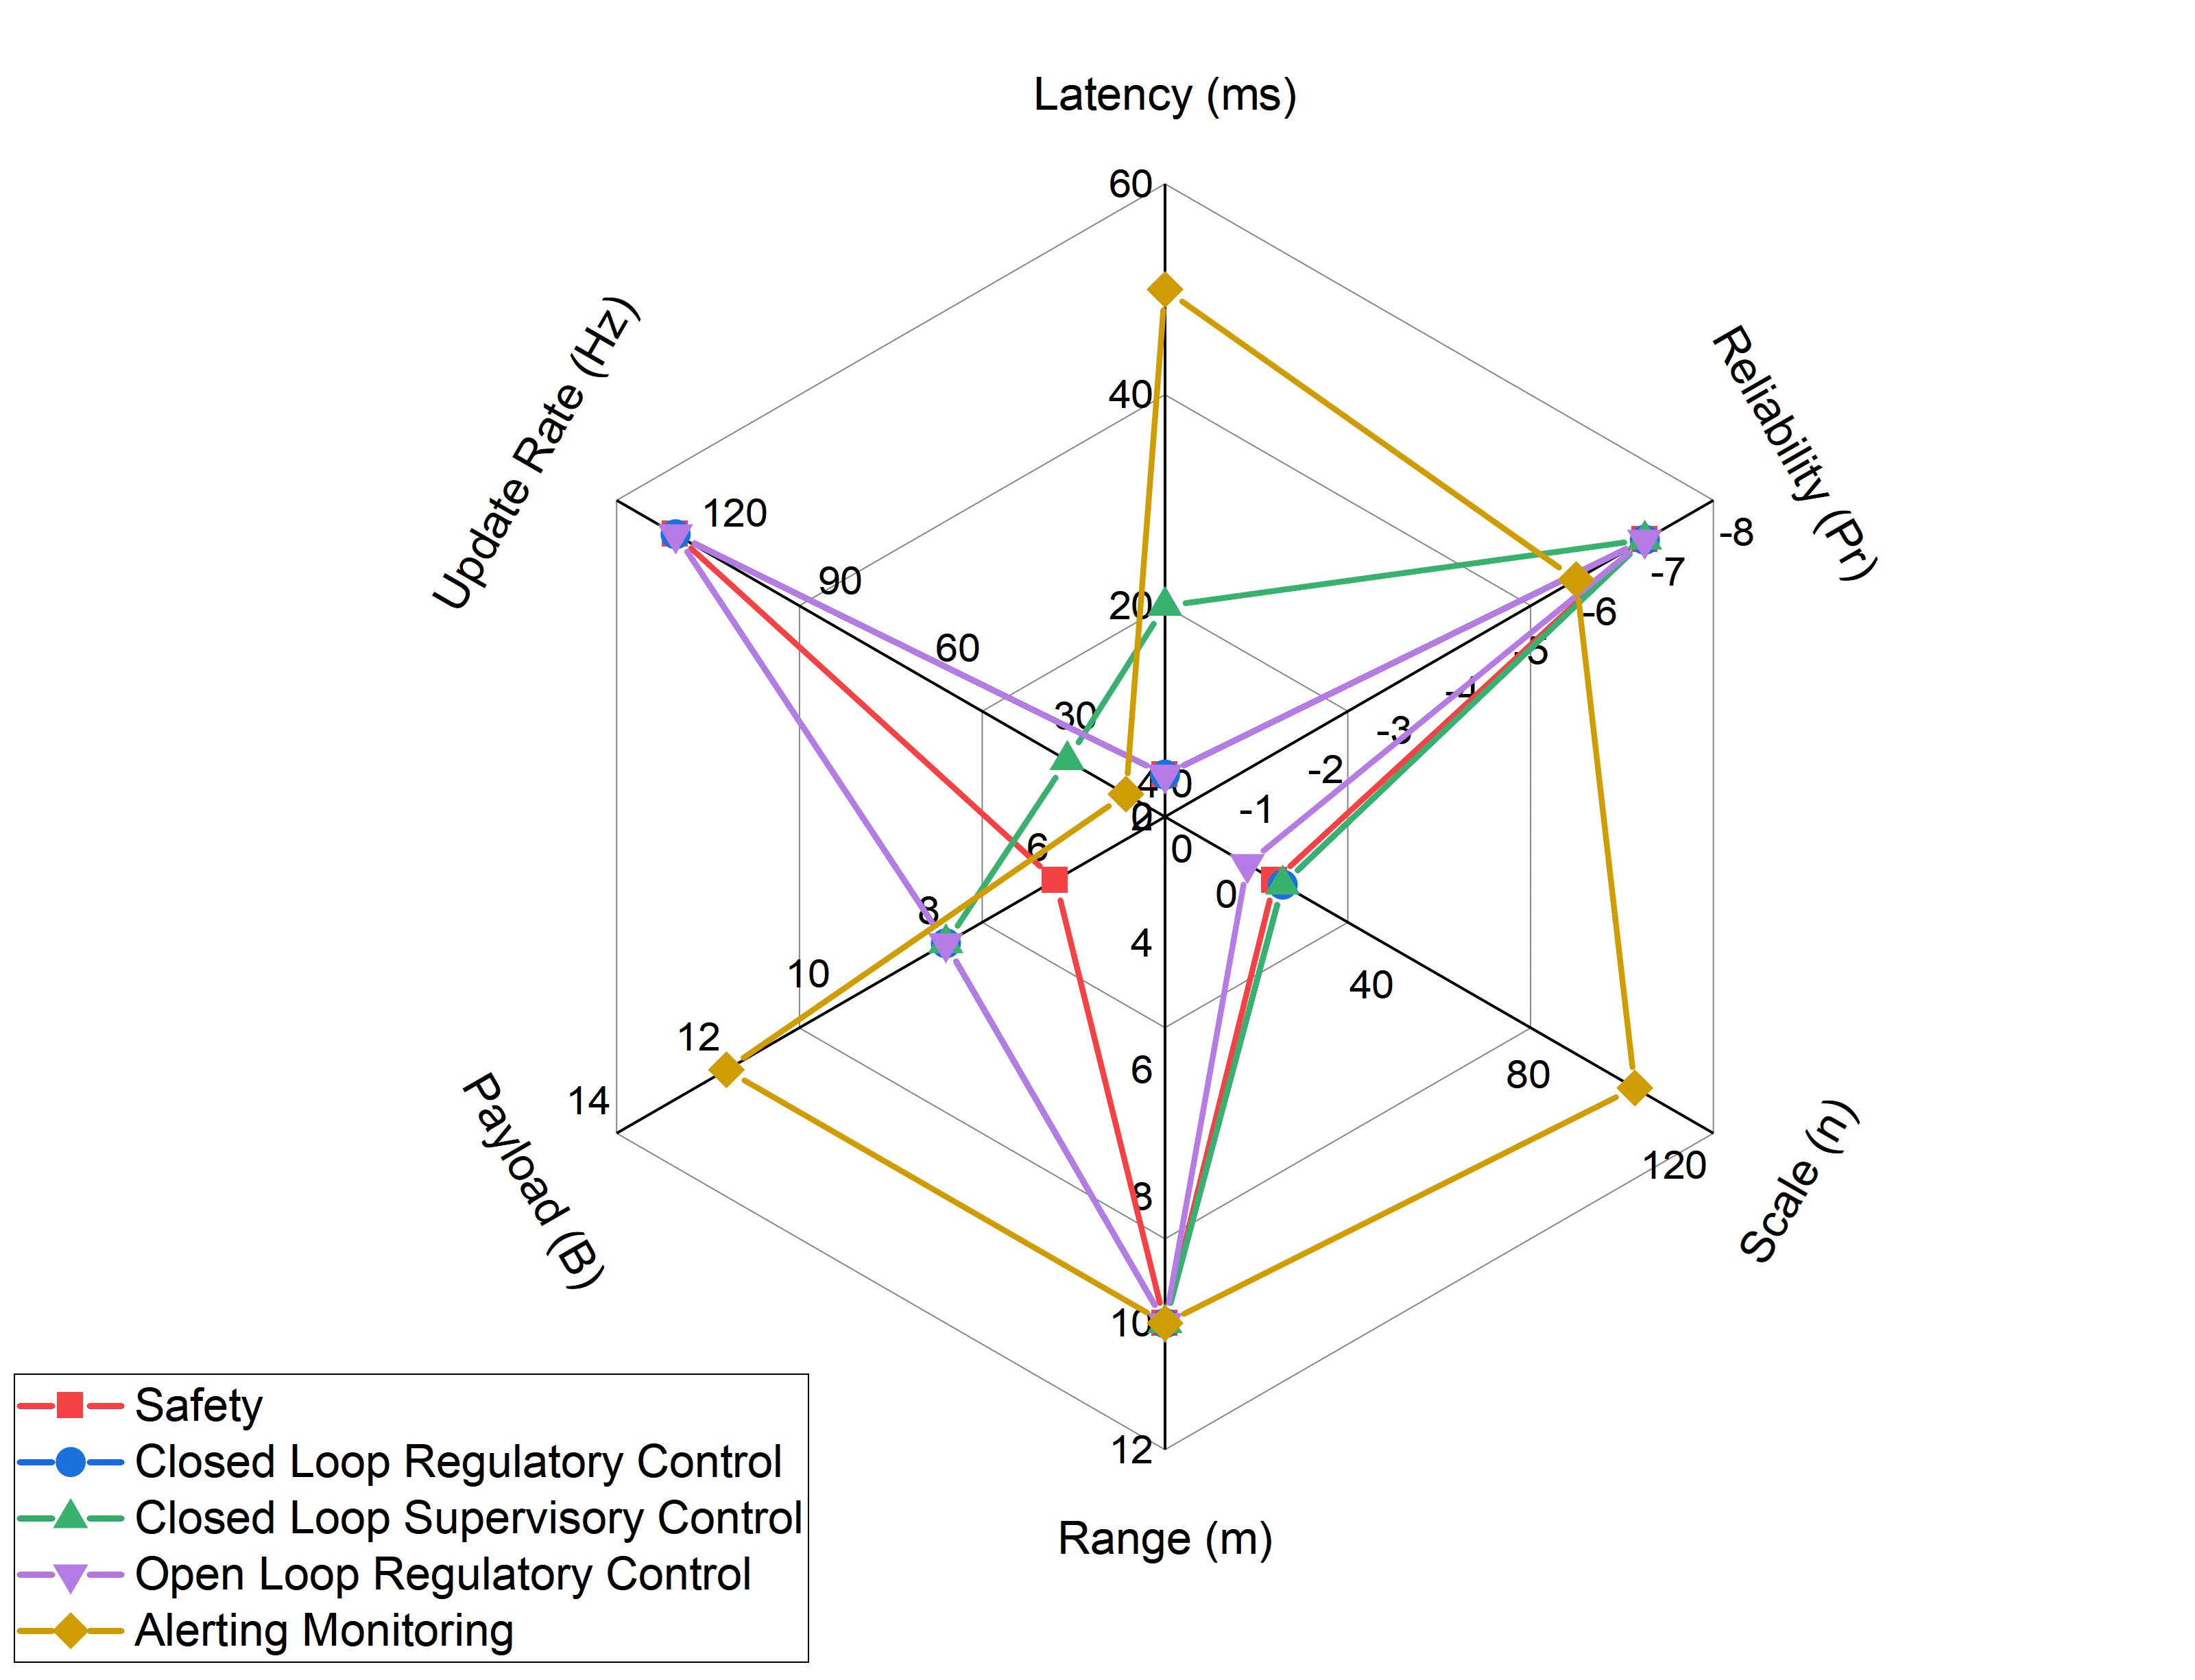
\includegraphics[width=\textwidth]{chapter-intro/diagrams/TypicalSpecs}
%	\caption{Typical performance specifications for industrial wireless use cases presented in~\cite{Montgomery2019}.}
%	\label{intro:fig:typicalspecs}
%\end{figure}
%
%
%\begin{figure}
%	\centering
%	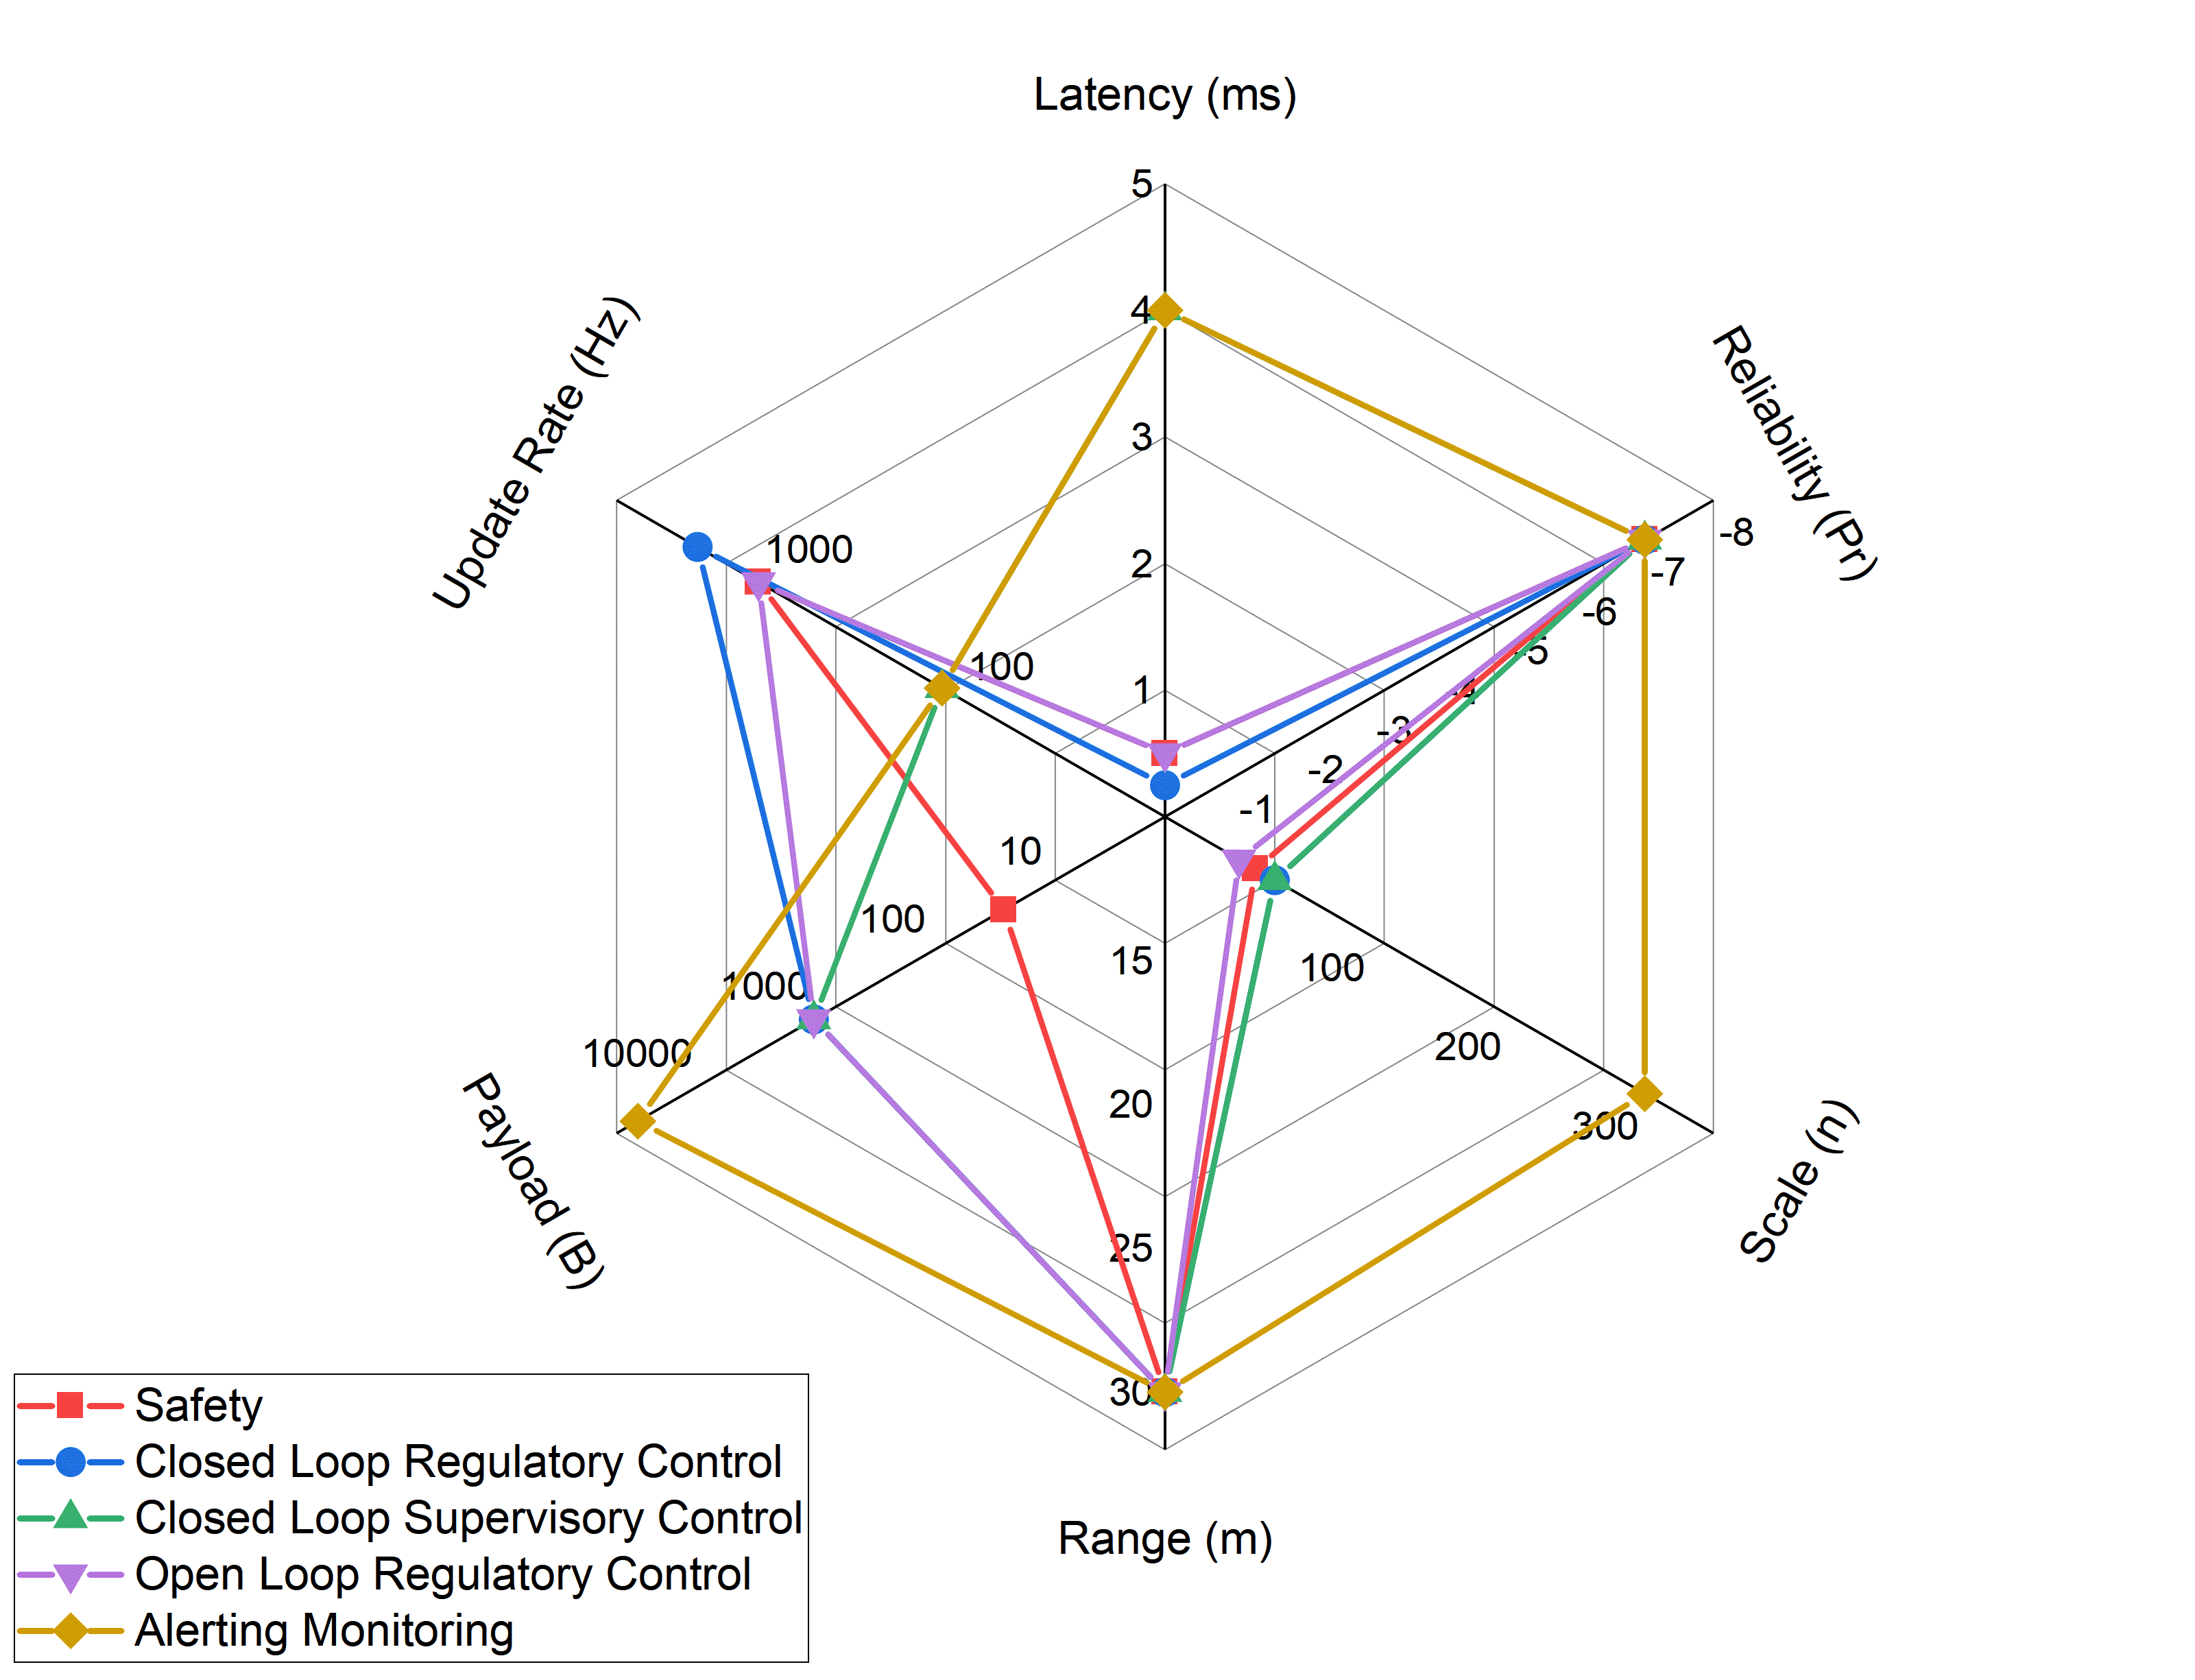
\includegraphics[width=\textwidth]{chapter-intro/diagrams/WorstSpecs}
%	\caption{Harshest expected performance specifications for industrial wireless use cases presented in~\cite{Montgomery2019}.}
%	\label{intro:fig:worstspecs}
%\end{figure}



\chapter{Systems Modeling}

\chapterintro*

This chapter provides a background to the reader in the state of the art in systems modeling.  Particular attention is given on the research done to how modeling tools and techniques are applied to the problem of the wireless smart manufacturing workcell, the components of such a workcell, or the data flows within the workcell.  The SysML model was developed to formalize and identify key components, interfaces, and constraints of the factory workcell.  The model developed is intended to include elements of both the physical system and network controlling behavior.  Therefore, the state of the art explored focuses on research performed to model both domains simultaneously capturing architecture and behavior.

\section{Modeling Languages} \label{sysml:sec:languages}

Current modeling work on factory work-cells is mainly aimed at defining and characterizing the subsystems, such as human staff, robots, and machine tools, in individual applications. By following blueprints (schematics) of production tasks, the work flow can be divided into separate assignments which are distributed by a task dispatch system to individual machines~\cite{IkeaBot}. Analytical models are thus obtained for performance analysis in work-cells. As an example, a mathematical model for real-time performance analysis of a gantry work-cell with robots is established with the timing and the randomness of tasks and disruptions are captured  \cite{8098604}. In \cite{OU2017212}, the same model is used to investigate the system natural properties such the system cycle and waiting times and to identify bottlenecks through studying the sensitivity of each machine. Similarly, the steady state analysis for production lines with uncertainties is performed through various decomposition methods~\cite{Colledani2013,doi:10.1080/00207543.2012.713137,doi:10.1080/00207540500385980}. In \cite{Colledani2013}, a decomposition method is presented for the analysis of continuous flow lines. The presented model is used to analyze flow lines with single and multiple failure mode machines and machines subject to aging and having up and down times. In \cite{doi:10.1080/00207543.2012.713137}, a model to evaluate the performance of transfer lines with unreliable machines and finite transfer-delay buffers is presented. A decomposition method is introduced to model the transfer line, using the general-exponential distributions instead of the exponential distributions to approximate the repair time distributions of the fictitious machines. In \cite{doi:10.1080/00207540500385980}, the authors present a model for evaluating the production rate and distribution of inventory of a closed-loop manufacturing system with unreliable machines and finite buffers. The model accounts for the different sets of machines that could cause blockage or starvation to other machines. In \cite{QChang,Liu2012}, the performance analysis modeling for serial production lines with disruptions is explored by studying the impact of each individual downtime event in terms of permanent production loss and financial cost. These analytical models generally work well for simple systems with small number of components or few interactions between various equipment. Also, the analytical models can be used to abstract industrial systems to understand various performance trends without studying various details. As a result, we introduce a comprehensive model that include network and production impacts on the industrial work-cell.  

Furthermore, the reconfigurable work-cell architecture is widely considered for automated manufacturing. The main advantage of reconfigurable work-cells lies in the flexibility of reconfiguration of work-cell components to adapt to varying production requirements where the assembly of the work cell is optimized for each specific task~\cite{CHEN2001199}. In the work-cell that hosts robots, robots are installed therein to allow for autonomous configuration within their workspace \cite{8023523,10.1007/978-3-319-65151-4_10,6059204}. Approaches and performance criteria for reconfigurable robotic systems have recent developments in control architectures to achieve various levels of reconfigurability \cite{Fulea}. The National Institute of Standards and Technology (NIST) has defined a Network of Things (NoT) model which can depict the structure of work-cells by a group of NoT building blocks and model the behaviors of individual components in a work-cell~\cite{NIST800-183}.  The NIST NoT model is focused primarily on sensor networks and the collection of data.  Actuation is cursorily noted, and, as such, cross-domain interactions between the physical system and the network are not addressed. Several other robotic work-cell architectures are discussed in the literature. In \cite{OpenArch}, a reference model for a control system functional architecture applied to open architecture robot controllers is presented. In \cite{CARPANZANO2007435}, a methodology to develop self-adaptive factory automation solutions is illustrated, using a novel modular simulation based method. With the increase in complexity and reconfigurability of work-cells, studying various production criteria and networks impacts requires introducing new models to capture these interactions and to be abstract enough to model different configurations and scenarios of industrial work-cells.  

In a work-cell model, data flows are used to capture the trajectory of system information exchange between work-cell components and identify their roles in specific operations~\cite{OpenArch}. For example, safety-related operations employ the vision system and various proximity sensors that generate proximity data and transmit them to the safety manager to define safety zones in an automotive assembly work-cell~\cite{safeeye}. 
In another example, data flows are enabled in a work-cell to capture human operator gestures from embedded cameras in human-robot collaborations~\cite{cobotcell}. These gestures can be later regenerated in simulators based on the transmitted position data from the field to optimize work-cell safety operations~\cite{gesture}. Currently, most of the work-cell information in these scenarios are transmitted by wired networks. Wireless networks have gained increasing interests to enable data flows in the highly connected work-cells. Wireless standard bodies have proposed their network reference models in factory environments which include the work-cell cases in the data-centric architecture~\cite{ETSI889, KPItable}. In these models, individual work-cells are treated as a subnetwork of field instruments attached with data aggregations that manage network connections and transfer data traffic to edge and cloud servers in various applications. Wireless connections are featured with flexible network topology to agree with a variety of transmission needs, especially in reconfigurable work-cells. Meanwhile, data traffic flows are characterized by select performance metrics, such as transmission latency and link reliability, to categorize industrial use cases~\cite{KPItable}. 

Current modeling efforts set the boundaries of their systems of study at the edge devices without further discussions on the impact of wireless performance on the operations of industrial systems. For example, the abstracted disruptions in \cite{QChang,Liu2012} that cause plant downtimes may include wireless network impacts which are not yet treated distinguishably with specific characteristics of wireless networks. As indicated by the earlier empirical studies~\cite{LIU2017412}, such physical systems may have different responses to network performance which will vary with the operational configuration such as the served ``application'' and the deployed control algorithms. In this paper, we incorporate the features of wireless communications networks into the modeling architecture of physical work-cells such that cross-domain interactions may be studied.  Prior to introducing the model for wireless incorporation, we first provide the reader an introduction to SysML in the following section.

\section{Systems Modeling Using SysML} \label{sysml:sec:systemsmodeling}

The goal of modeling a system is the capture of knowledge of a process in a simplified way~\cite{SysModel2004}. A secondary goal of a system model is to provide a level of abstraction that may allow for the discovery of new knowledge such as how two systems will interact. There are multiple ways of designing and presenting system models. Well-behaved systems can be represented by a system of equations using mathematical tools~\cite{SimModel1999}. Such models provide excellent constraint definition, but lack the semantics to describe architecture and detailed information flow.
Moreover, by deploying functional block diagrams, we are able to capture major functional components and flow of information or material. As shown in Fig.~\ref{sysml:fig:fbd-system}, a physical process interacts with a control system through a wireless network.  Measured values, $Y$, from sensors flow to the controller through a wireless network and arrive at the controller delayed and modified, $\bar{Y}$. Similarly, commands, $U$, flows from the controller to the actuators through the wireless network. Such diagrams may be used to model feedback control systems in which the origination and routing of information are immaterial for study. However, the architecture and interfaces remain at a very high level of abstraction making analysis difficult. In such cases, delay and loss using such tools are often modeled stochastically. Using architectural diagrams helps identify components, interfaces, and information flow. For factory systems, architectural block diagrams are often manifested as schematics. However, such diagrams have their own limits in industrial practices. On one hand, they lack the semantics necessary to describe the constraints that formal equations and functional block diagrams offer. Meanwhile, they also lack the capability of capturing behaviors or complex interactions between the physical system and the information infrastructure such as a wireless network. 

\begin{figure}
	\centering
	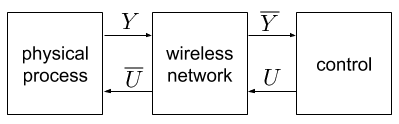
\includegraphics[width=0.65\columnwidth]{./chapter-sysml/diagrams/fbd-system}
	\caption{Functional block diagram of a cyber-physical system in which a physical process and an automation system interact through a wireless network.}
	\label{sysml:fig:fbd-system}
\end{figure}

An alternative to schematic diagrams is SysML~\cite{SysML2017}. SysML is a general purpose modeling language that is often used for model-based systems engineering (MBSE) practice within industrial systems~\cite{MBSEandSysML}. SysML provides structural, behavioral, and parametric semantics for the analysis of complex systems. For examples, systems analysis using SysML enables capturing and communicating system requirements and design which include hardware, software, firmware, information flows, and processes with graphical notations. Within the factory automation industry, engineers are adopting SysML in the form of MBSE to develop realizable operational models of the factory and data flow processes. MBSE models address verification of design through executable simulations depending on the modeling tool.  The SysML specification is defined in~\cite{SysML2017}.  In SysML, the basic semantic constructs of the language are Packages, Blocks, Ports, Interfaces, and Constraints, in addition to the constructs provided by the Unified Modeling Language (UML). Packages are logical grouping of model elements. Package relationships are captured using the package diagram (PKG). Relationships of these constructs are captured in the block definition diagram (BDD).  The internal composition and connectivity of parts are captured in the internal block diagram (IBD). SysML includes other types of diagrams and semantic constructs that are not required for this analysis and are not explained here. The SysML model is comprehensive; however, the size and number of diagrams within the model are too extensive to include within this paper.  Therefore, the reader is encouraged to explore the SysML model defined in~\cite{SysML.Candell2018}.  A useful primer on SysML may be found in~\cite{Friedenthal2015.SysML}. 

Examples of the use cases and methodologies of using different graphical models for the analysis of manufacturing systems are explored in~\cite{Lutjen2015.GramosaMethod,Luder2011.GraphicalModeling,Jia2013.GraphicalModeling,Alvarez2013.GraphicalModeling}.  In~\cite{Quinsat2017.SysML}, SysML is used to capture both composition and behavior of an additive manufacturing work-cell.  A survey of applying graphical modeling languages in capturing information flows within a product service system which may be applied to manufacturing enterprises~\cite{Durugbo2011.GraphicalModeling}.  Our approach compliments these previous examples by combining the operational and wireless information transport systems together in a single model, thereby facilitating a single model that may be used for simulation and other systems engineering analyses.

While various architectures for the work-cell exist as exemplified in the literature, a common language and framework for communicating architecture and information flow has not been established for cross-domain interactions between the manufacturing system and its supporting communication networks.
SysML contains the semantics for such engineering capture and provides an industry accepted language for communicating composition, interfaces, and information flow. Moreover, SysML provides the semantics for assigning properties to any model element such that those properties are made  available for analysis using other tools such as Prot\'eg\'e \cite{StanfordUniversity.Protege} and the Web Ontology Language (OWL) \cite{W3C2012.OWL}.
It is important to understand that while SysML provides semantics for a formal capture of architecture, information flow, and parametric constraints, it may also be used for a higher-degree of abstraction provided by the functional block diagrams.  

\chapter{Use of Databases for Performance Analysis}

\chapterintro*

\blindtext

Multiple surveys about GDBs have been presented to describe the associated models, tools, and their features in~\cite{Angles:2008:SGD:1322432.1322433,7148480,GDB_overview}. Also, examples of applications and implementations of GDBs are presented in~\cite{modern_models} to show their use on enterprise data, social networks, and determining security and access rights. It was found that GDBs provide the much needed structure for storing data and incorporating a dynamic schema. On the other hand, query languages are used to extract data including traversing the database, comparing nodes properties, and subgraph matching~\cite{Wood2012QueryLF}. The performance of different GDB tools and methodologies is analyzed and compared in~\cite{Jadhav2015ComparativeAO,Macko:2013:PIG:2485732.2485750}. Multiple comparisons in these articles have shown improved performance of Neo4j in the general features for data storing and querying, and data modeling features such as data structures, query languages and integrity constraints. 

Furthermore, industrial data analytics play an essential role in achieving the smart factory vision and improving decision-making in various industrial applications. Five main industrial data methodologies are studied including highly distributed data ingestion, data repository, large-scale data management, data analytics, and data governance~\cite{DBLP:journals/corr/abs-1807-01016}. Industrial data processing offers valuable information about various sections of industrial applications including inefficiencies in industrial processes, costly failures and down-times, and effective maintenance decisions~\cite{JLee}. In~\cite{4}, a platform for performing industrial big data analysis is presented where the performance requirements are introduced to achieve a cost-effective operation. Various other frameworks for industrial data analysis can be found in~\cite{5,6}, where the importance of using data analysis in decision making is emphasized.

Due to its advantages including scalability, efficiency, and flexibility, NoSQL databases are a popular alternative to relational databases in the case of large amounts of data in various applications~\cite{doi:10.1108/17440081311316398}. The GDB is a kind of NoSQL database approaches that additionally handles complex relationships~\cite{8123475}. GDBs are widely adopted in various industry-related applications and use cases such as network operations, fraud detection, and asset and data management~\cite{top5}. Relationships in social networks have been modeled using a GDB for structural information mining and marketing~\cite{Gomez-Rodriguez:2012:IND:2086737.2086741}. On the other hand, business solutions for scenarios with multiple large data sources require distributed processing in decision making for various problems such as fraud detection, trend prediction, and product recommendation~\cite{Skhiri2013}.


\chapter{Machine Learning in Performance Estimation}

\chapterintro*

\blindtext

In the literature, two types of interference signals are considered, namely, intentional or unintentional interference. Methods to estimate, avoid, or mitigate interference are required for the deployment of reliable and deterministic IWSs. Machine learning has been widely used to detect and estimate interference information to enhance the performance of interference managment algorithms.  

The interference analysis in cyber-physical systems (CPSs) has been considered in multiple works for various scenarios. In~\cite{8639006}, in-network interference mitigation techniques are discussed for ultra reliable low-latency wireless communications systems. The paper focused on mutual interference mitigation in an industrial automation setting, where multiple transmissions from controllers to actuators interfere with each other. In \cite{Kumar2019}, an interference mitigating receiver architecture is proposed. The application scenarios are smart homes and modern factories where dense wireless communications devices exist. Moreover, in~\cite{Bhushan2014.NetworkDesensUsingIntfCancellation}, interference cancellation of transmissions from neighboring cells in a 5G cellular network is presented. In~\cite{Gomes2017.LQEinWSNs}, a method using a dedicated node for link quality estimation (LQE)  obtained through received data packets to identify interference and multi-path without introducing additional traffic is presented. In~\cite{Baccour2012.SurveyOnLinkEstimation}, a taxonomy of channel link quality techniques is presented providing a valuable survey on LQE algorithms and asserting the importance of link quality estimation in IWSs. In~\cite{Frounhoffer.Troubleshooting}, failure analysis and wireless network troubleshooting are performed whenever the CPS is not functioning properly. Interference analysis is one major part of the troubleshooting procedure which is performed through traffic patterns and wireless spectrum analysis. Also, in~\cite{NIST.InterfCoexCritical}, the use of spectrum analysis for interference detection and estimation is proposed for IWSs. 

On the other hand, intended interference (i.e., jamming) can lead to service denial or poor performance in wireless networks. In~\cite{8631535}, a literature review was presented which includes an overview of recent research efforts on networked control systems under denial-of-service attacks such as jamming attacks in wireless channels. One of the discussed challenges is how to achieve ultra-reliable low-latency "signalling" within industrial applications. In~\cite{Cetinkaya_2019}, a discussion is also provided on the recent developments concerning the design of attack-resilient control and communication protocols. Generally, a jamming attacker can block transmission of packets by emitting strong interference signals to a wireless channel \cite{1637931,5473884}. Jamming attacks can target various wireless technologies and hence can become a major concern for control systems, since they are easy to launch \cite{5473884}. It was shown in \cite{10.1007/978-3-319-07788-8_40} that off-the-shelf hardware can be used for generating jamming attacks on wireless networks. In cases of physical-layer attacks, the jamming attacker targets a frequency band and is not required to follow the wireless protocol where it can cause a decrease in the SIR thus preventing the receiver from successfully detecting transmitted packets \cite{10.1007/978-3-319-07788-8_40}. In the case of MAC-layer attacks, both the packet sender and the jamming attacker operate on the same channel; the jamming attacker’s goal is to cause packet collisions.
In~\cite{8726803}, the authors evaluated the CPSs resilience to jamming attacks that disrupt wireless communications. They considered three jamming strategies which are the constant, random, and protocol-aware jamming. They showed through experimental results that various CPS control schemes are susceptible to constant and random jamming while the time-triggered control schemes are susceptible to protocol-aware jamming. Moreover, resilience of CPSs is also considered in~\cite{6425868,DEPERSIS2014134,7402971,7575630} where periodic jamming is considered in \cite{6425868} while the jamming strategy in~\cite{DEPERSIS2014134,7402971,7575630} is neither known nor pre-fixed. 

Machine learning has been used for detection and estimation of jamming attacks. In~\cite{Chen2019}, an unsupervised machine learning algorithm based on a multi-layer autoencoder is used to extract the interference source spectrum features. These features are then used to distinguish interference sources type and location without labeling measured data. In~\cite{7911887},  an unsupervised approach using a recurrent neural network to detect anomalies in the CPS performance and identify attacked sensors. In~\cite{Junejo2016DataDP}, a behavior based machine learning intrusion detection approach  is proposed to detect attacks at the physical process layer. The results are validated through experimental study of a real modern water treatment facility. In~\cite{Beaver:2013:EML:2584691.2584722}, the viability of machine learning methods in detecting the new threat scenarios of command and data injection is assessed. In that work, command and control communications in a critical infrastructure setting are monitored and vetted against examples of benign and malicious command traffic to identify potential attack events. In~\cite{6900095}, the authors assessed discriminating types of power system disturbances through machine learning by detecting jamming attacks. They evaluated various machine learning methods as disturbance discriminators and discuss the practical implications for deploying machine learning systems as an enhancement to existing power system architectures.

Therefore, in the literature, it was shown that LQE is one important but insufficient aspect of assessing the impact of link quality on a CPS. We assert that by jointly observing the performance of the physical and wireless components of a CPS,the complete perspective of the quality of the wireless link and its impact on physical performance can be obtained. Since interference is such an important topic in the wireless CPS, we are motivated to propose a method that simultaneously (1) makes observations of the physical system using ground truth measurements, and (2) infers the quality of the wireless communication system in terms of SIR using an experimental model of a relevant use case found in industry.
